
\chapter{Belle~II}
\label{chap:belleIIDet}

\begin{figure}[htb]
	\centering
		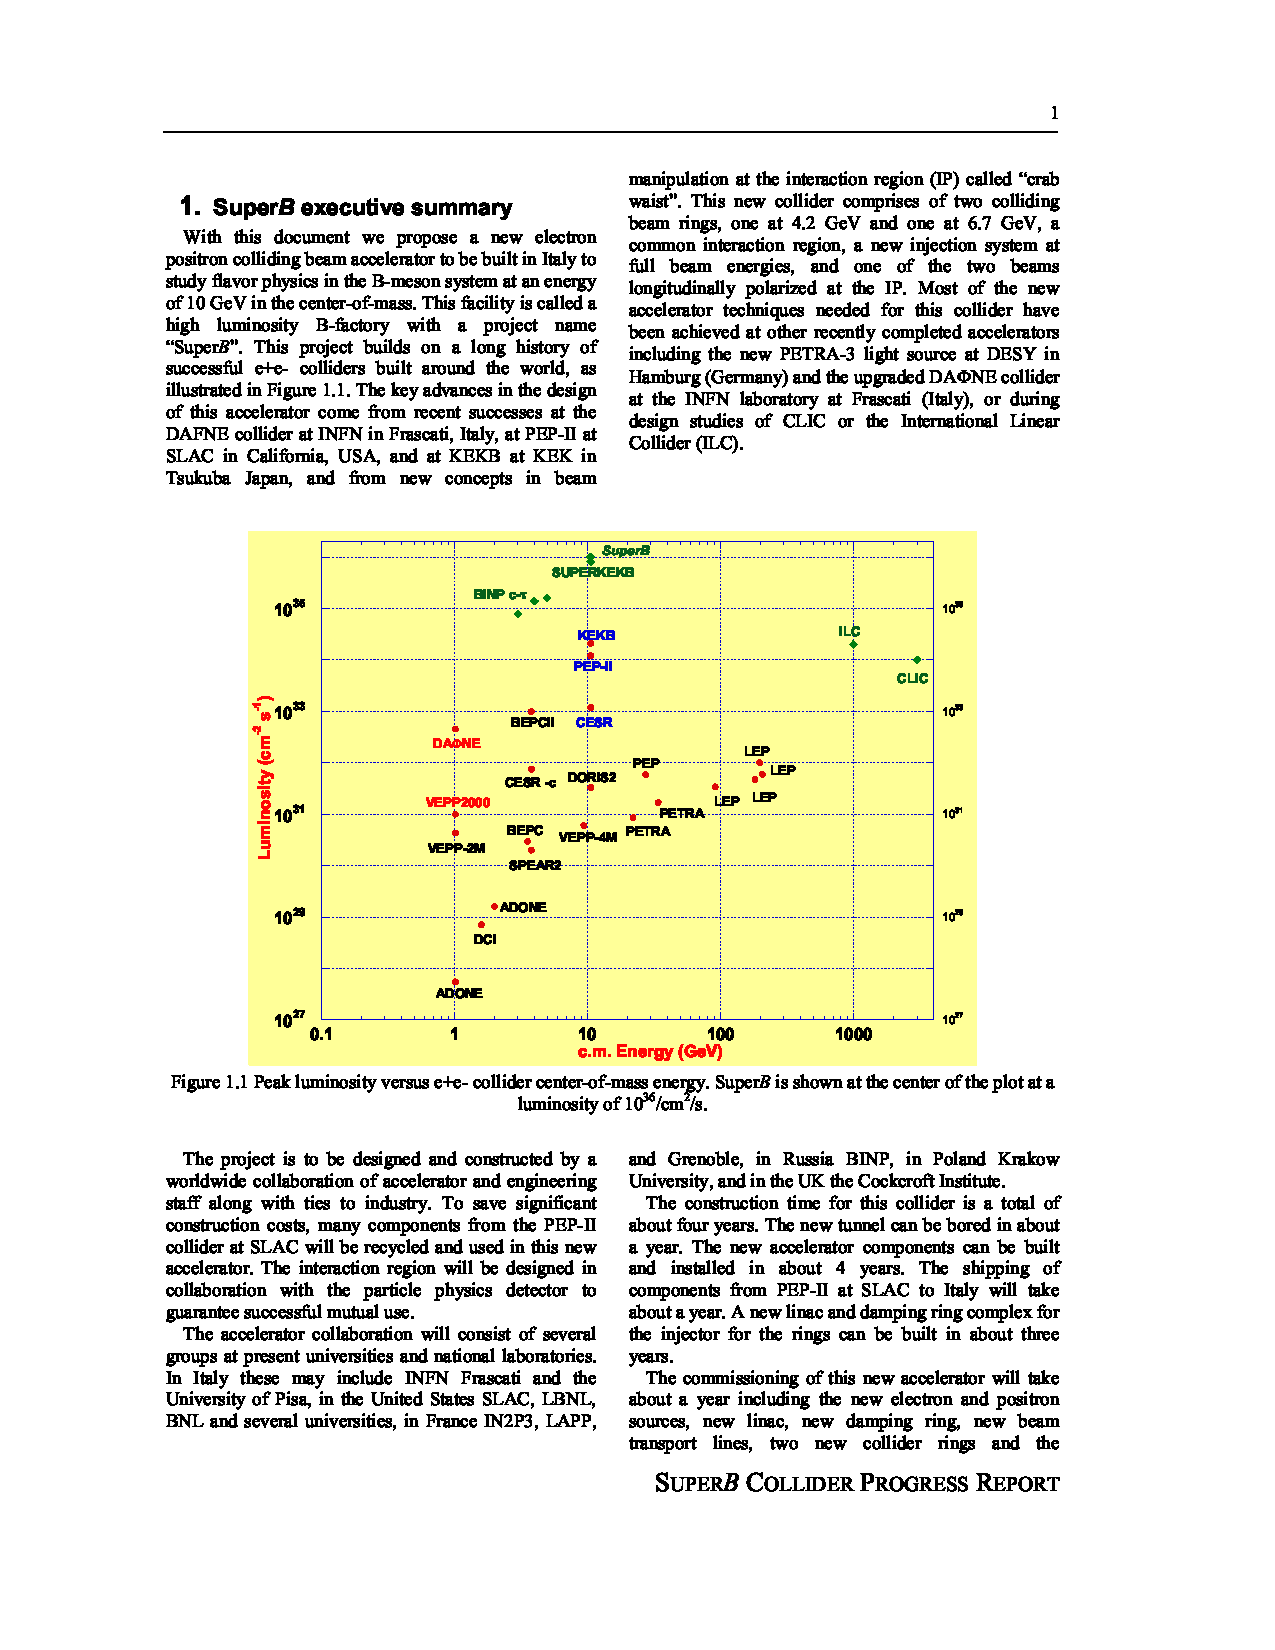
\includegraphics[trim=100 280 150 250,clip=true, scale=0.9]{images/CMvsLum.pdf}
	\caption[Peak luminosity vs centre of mass energy for various collider experiments]{Peak luminosity vs centre of mass energy for various collider experiments~\cite{superbaccelerator}.}	
	\label{fig:CMvsLUM}
\end{figure}

SuperKEKB is a super B-factory which has been built at the KEK high energy laboratory in Tsukuba, Japan. It consists of the SuperKEKB asymmetric \epem collider, storage rings, and the Belle~II detector. The collider will run at a centre of mass energy of 10.58 GeV, which is the mass of the $\Upsilon(4S)$  $b\bar{b}$ resonance. With a luminosity goal of  8$\times10^{35}$ cm$^{-2}$s$^{-1}$, SuperKEKB will be the highest luminosity \epem collider ever built (see Fig \ref{fig:CMvsLUM}).

\section{Physics motivation}

	Electron-positron B-factories are a type of collider experiment that use \epem colliders with high luminosity to make precision measurements of particle interactions involving mesons containing b quark and c quarks as well as tau leptons. Belle~II is a next generation \epem B-factory, called a super-B factory. The centre of mass energy of Belle~II is just enough to produce the $\Upsilon(4S)$ resonance, but the majority of collisions produce other particles, allowing investigation of processes involving charm quarks and tau leptons. Measurements of CP-violation, in which matter and antimatter behave differently, will be made in Belle~II. Due to the precision of the measurements that will be made at Belle~II, small deviations from the Standard Model of particle physics can be detected, which may be a sign of new physics. Searches for other sources of new physics (such as dark matter) are possible through \epem collisions. Rare and forbidden decays can also be measured, which is another sign of new physics~\cite{GrantProp}.


\section{SuperKEKB Collider}
\label{sec:SKB}




SuperKEKB (see Fig \ref{fig:SKB}) is an asymmetric \epem collider built at the KEK high energy laboratory in Tsukuba, Japan. It has been constructed in the same tunnel as its predecessor KEKB, but has many upgrades to increase the luminosity to 8$\times10^{35}$cm$^{-2}$s$^{-1}$, 40 times the luminosity achieved in KEKB. Other beam parameters are presented in Table \ref{tab:SKBBEAM}.

Electrons are produced and accelerated to 7.0 GeV by a linac. Before acceleration, some of the electrons produced are used to generate positrons by irradiation of a tungsten target located in the middle of the linac. Due to the nature of this production, the emittance of the positron beam will be very large. To mitigate this the positron beam will be pulled off the linac and injected into a damping ring. After damping, the positrons are returned to the linac and accelerated to 4.0 GeV. Both rings have a circumference of 3.0 km.

Due to the higher energy of the electron beam, the centre of mass of Belle~II is boosted in the direction that the electron beam is travelling. This boost allows the decay time of the particles produced in the interaction to be dilated by special relativity, enabling time-dependant measurements of CP-violation. 

The electrons and positrons are continuously injected into the high energy ring (HER) and low energy ring (LER). This continuous injection allows the beam current to remain constant, allowing a high luminosity~\cite{BELLE2TDR, ohnishi2013accelerator}.


\begin{table}[htb]
	\centering
	\begin{tabular}{ lcc }
	&	LER	&	HER	\\	\hline \hline
Accelerates	&	e+	&	e-	\\	
Beam Energy (GeV)	&	4.0	&	7.0	\\	
Beam Current (A)	&	3.60	&	2.62	\\	
Horizontal Beam Size ($\mu$m) & 10.2 & 7.75 \\
Vertical Beam Size (nm) & 59  &  59 \\
Number of Bunches	&	\multicolumn{2}{c}{2503}			\\	
Luminosity (cm$^{-2}$s$^{-1}$)	&	\multicolumn{2}{c}{8$\times 10^{35}$}			\\	
Residual beam pipe pressure (nTorr) &  \multicolumn{2}{c}{10}  \\ \hline

	\end{tabular}
	\caption[SuperKEKB beam parameters]{SuperKEKB beam parameters~\cite{BELLE2TDR}.}
	\label{tab:SKBBEAM}
\end{table}



\section{Belle~II detector}

The Belle~II detector is composed of eight subdetectors (see full schematic in Fig \ref{fig:BELLE2}). The inner and outer radii (measured from the beam line axis) as well as the angular acceptance of each subdetector are shown in Table \ref{tab:belleIIaccept}.  Belle~II uses a cylindrical coordinate system to define positions. The $z$-axis runs through the solenoid axis, in the direction that the electron beam travels. Positive $z$ is referred to as the forward direction, and negative $z$ is the backward direction. $x$ is the direction towards the outside of the SuperKEKB ring, and $y$ is upwards. $\phi$ is the azimuthal angle around $z$, and $\theta$ is the zenith angle with respect to $z$.


 This section describes each subdetector, starting at the innermost.

\begin{figure}[htb]
	\centerfloat
		\includegraphics[scale=0.6]{images/SKEKb_key}
	\caption[The SuperKEKB \epem collider]{The SuperKEKB \epem collider. The rings have a circumference of 3 km~\cite{SKBgroup}.}
	\label{fig:SKB}
\end{figure}




\begin{sidewaysfigure}
	\centering
	\includegraphics[width=\paperwidth]{images/Belle-llTopview_simple}
	\caption[The Belle~II detector]{Cross section of the Belle~II detector. The forward direction is on the right, and is the direction the electron beam travels. The whole detector is 5 m tall, and approximately symmetric in $\phi$~\cite{BELLE2TDR}.}
	\label{fig:BELLE2}
\end{sidewaysfigure}


\begin{table}[ht]
	\centering
	\begin{tabular}{ lcccc }
Subdetector	&	Inner Radius (mm)	&	Outer Radius (mm)	&	$\theta_{min}$ (deg)	&	$\theta_{max}$ (deg)	\\	\hline \hline
PXD	&	14	&	22	&	17	&	150	\\	
SVD	&	38	&	140	&	17	&	150	\\	
CDC	&	160	&	1130	&	17	&	150	\\	
TOP	&	1190	&	1243	&	32	&	128	\\	
ARICH	&	420	&	1140	&	13	&	34	\\	
Forward ECL	&	1378	&	420	&	12.3	&	32	\\	
Barrel ECL	&	1244	&	1617	&	32	&	130	\\	
Backward ECL	&	417	&	1392	&	130	&	155.1	\\	
BKLM	&	1952	&	2475	&	45	&	125	\\	
EKLM	&	1248	&	2475	&	20	&	145	\\	\hline

	\end{tabular}
	\caption[Inner and outer radii, and angular acceptances of Belle~II subdetectors]{Inner and outer radii, and angular acceptances of Belle~II subdetectors, measured from the forward direction. The detectors are approximately symmetric in $\phi$.}
	\label{tab:belleIIaccept}
\end{table}



\subsection{Vertex Detector}
\label{sec:VXD}

	Belle~II's vertex detector (VXD) is made up of two tracking subdetectors. The inner detector is the pixel detector, which is surrounded by the silicon vertex detector.

\subsubsection{Pixel Detector}
\label{sec:PXD}

	The \textbf{P}i\textbf{X}el \textbf{D}etector (PXD) is wrapped around the beampipe. This subdetector is made up of two cylindrical layers containing solid state pixel cells. The inner cylinder has a radius of 1.4 cm and has eight segments, while the outer cylinder has a radius of 2.2 cm and has 12 segments. The PXD contains about 8 million individual pixel cells \cite{BELLE2TDR, schieck2013depfet}.


\subsubsection{Silicon Vertex Detector}
\label{sec:SVD}

	The \textbf{S}ilicon \textbf{V}ertex \textbf{D}etector (SVD) surrounds the PXD. Its purpose is to measure decay vertices, particularly those of B decays. It consists of four layers containing strips of double sided silicon detectors. Due to the smaller Lorentz boost of Belle~II compared to Belle, there is less separation between the B decay vertices; however, the beampipe of Belle~II is smaller, which allows the Belle~II SVD to have improved performance compared to Belle \cite{BELLE2TDR}.

	


\subsection{Central Drift Chamber}
\label{sec:CDC}

	The \textbf{C}entral \textbf{D}rift \textbf{C}hamber (CDC) surrounds the VXD. It provides three important functions: reconstruction of tracks and momentum measurements of charged particles, particle identification through energy loss within the gas volume, and efficient and reliable triggers for charged particle tracks. The CDC is a cylindrical chamber, with over 14,000 sense wires strung along the length of the cylinder. It is filled with He-C$_2$H$_6$. As charged particles traverse the gas, they create tracks of ionization, which are detected by the sense wires. The path of the particle through the CDC can then be reconstructed. The CDC is immersed in a 1.5~T solenoidal magnetic field, parallel to the beampipe. This allows the CDC to act as a large magnetic spectrometer ~\cite{BELLE2TDR}.


\subsection{Particle ID}
\label{sec:PAID}

	Belle~II has two particle ID (PID) detectors: the TOP and the ARICH. The TOP is in the central region of Belle~II, while the ARICH is in the forward region.

\subsubsection{Time of Propagation Counter}
\label{sec:TOP}

	The barrel PID detector is known as the \textbf{T}ime \textbf{O}f \textbf{P}ropagation (TOP) counter. Its purpose is to improve Belle~II's ability to distinguish between kaons and pions. The counter measures the time of propagation of Cherenkov photons internally reflected within a quartz radiator. The detector consists of 16 modules which run parallel to the axis of Belle~II. Each module is made up of a single rectangular bar of quartz with a focusing mirror on one end and a photomultiplier tube (PMT) on the other end. As particles traverse the crystal, Cherenkov light is produced in the crystal. This light is reflected down the bar into the PMT. Information about the incident particle's ID can be inferred from this light~\cite{BELLE2TDR}.


\subsubsection{Aerogel Ring-Imaging Cherenkov detector}
\label{sec:ARICH}

	Sandwiched between the CDC and the forward ECL end-cap is the \textbf{A}erogel \textbf{R}ing-\textbf{I}maging \textbf{CH}erenkov (ARICH) detector. Its purpose is to identify kaons and pions over most of the momentum range and to discriminate between pions, muons, and electrons at momenta below 1 GeV/c. The detector consists of an aerogel radiator where charged particles create Cherenkov photons, an expansion volume where the photons propagate so that distinctly measurable rings can form, and an array of photon detectors (known as HAPDs: \textbf{H}ybrid \textbf{A}dvanced \textbf{P}hoto-\textbf{D}etector) which measure the Cherenkov rings~\cite{BELLE2TDR}.



\subsection{Electromagnetic Calorimeter}
\label{sec:ECL}

	The \textbf{E}lectromagnetic \textbf{C}alorimeter (ECL) has several tasks: high efficiency photon detection, precise photon energy and angular measurements, identification of electrons, trigger signalling, luminosity measurements, and (with the $K_{L}^0$ and $\mu$ detector) K$_L^0$ measurement. Note that all particles will potentially lose some energy that is measured in the ECL, which will contribute to particle identification. The ECL is composed of 8,736 crystals of thallium doped caesium iodide (CsI(Tl)) and is divided into three parts: the forward end-cap containing 1,152 crystals, the barrel containing 6,624 crystals, and the backward end-cap containing 960 crystals. Apart from the electronics the entire calorimeter is the same as was used in the Belle experiment. Each crystal is roughly 30~cm in length, which corresponds to 16 radiation lengths. The crystals have a cross section of $\sim5~\mathrm{cm}\times5~\mathrm{cm}$.

Attached to the end of each crystal is a diode that measures the scintillation light produced by the crystal, which is proportional to the energy deposited in that crystal. The front-end electronics of the ECL have been upgraded since Belle and now read and process the waveforms using a Field Programmable Gate Array (FPGA), producing time and amplitude \cite{BELLE2TDR}.


\subsection{K$_L^0$ and $\mu$ detector}
\label{sec:KLM}


The outermost detector system is the K$_L^0$ and $\mu$ detector (KLM), which is made of three components: two end-caps (EKLM) and a barrel (BKLM). These components consist of alternating layers of 4.7~cm thick iron plates and active detector material. In the barrel, the active material is made up of glass-electrode resistive plate chambers (RPC). The end-caps have to deal with a much higher background flux, so the active materials there are scintillators. The barrel KLM covers 45$^{\circ}$ to 125$^{\circ}$ and is made up of 15 layers, providing 3.9 interaction lengths of material. The end-caps extend this range from 20$^{\circ}$ to 155$^{\circ}$. The forward end-cap has 12 layers, while the backward end-cap has 14 layers~\cite{BELLE2TDR}.

\subsection{Shielding}

	In order to mitigate the effects of beam backgrounds, shields composed of polyethylene with 5\% boron and lead are installed inside the forward and backward ECL. The polyethylene and boron absorb neutrons and the lead absorbs photons and electrons. In addition to this, the ARICH has a small neutron shield made of polyethylene built into it.

\subsection{Neutron Damage to Belle~II Subdetectors}



	The readout electronics of each subdetector are all silicon based. 3.05\% of silicon is composed of the $^{30}$Si isotope, which can be transmuted into phosphorous by this reaction:
\begin{equation}
	{^{30}\mathrm{Si} + \mathrm{n}\rightarrow~^{31}\mathrm{Si}+\gamma \rightarrow~^{31}\mathrm{P}+\beta^{-}+\gamma}
\end{equation}
which introduces an n-type dopant into the silicon, altering its electronic properties. Additionally, there is lattice damage caused by recoil. Other silicon isotopes, $^{28}$Si and $^{29}$Si will also absorb neutrons, but since they remain silicon, they do not alter the electronic properties other than introducing lattice damage~\cite{young1978radiation}.

The simulated neutron flux in each Belle~II subdetector is presented in Chapter~\ref{chap:Conseqences}. The unscaled figures are for the basic simulation and the scaled figures are after the analysis presented in this dissertation. Expected neutron fluxes are on the order of $10^9$ neutrons cm$^{-2}$yr$^{-1}$ for most detectors, with the vertex detectors having a higher flux, and the KLM detectors having a lower flux. Some detectors are more sensitive to neutron background, particularly the ARICH and TOP detectors and the electronic components of the other detector readouts.




%Several subdetectors are particularly sensitive to neutron damage: the ARICH and the TOP. 

%ARICH: Noise increases. Has additional shielding















